\documentclass[12pt,a4paper]{article}

\setlength{\textwidth}{165mm}
\setlength{\textheight}{240mm}
\setlength{\parindent}{0mm} % S{\aa} meget rykkes ind efter afsnit
\setlength{\parskip}{\parsep}
\setlength{\headheight}{0mm}
\setlength{\headsep}{0mm}
\setlength{\hoffset}{-2.5mm}
\setlength{\voffset}{0mm}
\setlength{\footskip}{15mm}
\setlength{\oddsidemargin}{0mm}
\setlength{\topmargin}{0mm}
\setlength{\evensidemargin}{0mm}
\usepackage{multicol}
\usepackage{blindtext}
\usepackage[all]{xy}
\usepackage{graphicx}    % For grafik (billederfiler)
\usepackage[T1]{fontenc} % For at blande \textsc{} med \textbf{}
\usepackage[utf8]{inputenc}
\usepackage{amsfonts,amsmath,amssymb}
\usepackage{eucal}
\usepackage{enumerate}  
\usepackage{hyperref}
\usepackage{url}
\usepackage{mathptmx}
\usepackage{multirow}
\usepackage[dvipsnames,usenames]{color}
\usepackage{tabularx,colortbl,xcolor}
\usepackage{listings}
\usepackage{color}
\usepackage{amsmath}
\usepackage{xcolor}

\definecolor{KU-red}{RGB}{144,26,30} 
\definecolor{dkgreen}{rgb}{0,0.6,0}
\definecolor{gray}{rgb}{0.5,0.5,0.5}
\definecolor{mauve}{rgb}{0.58,0,0.82}

\lstset{frame=tb,
  language=Java,
  aboveskip=3mm,
  belowskip=3mm,
  showstringspaces=false,
  columns=flexible,
  basicstyle={\small\ttfamily},
  numbers=none,
  numberstyle=\tiny\color{gray},
  keywordstyle=\color{blue},
  commentstyle=\color{dkgreen},
  stringstyle=\color{mauve},
  breaklines=true,
  breakatwhitespace=true,
  tabsize=3}

\DeclareSymbolFont{usualmathcal}{OMS}{cmsy}{m}{n}
\DeclareSymbolFontAlphabet{\mathcal}{usualmathcal}
\DeclareSymbolFont{letters}{OML}{txmi}{m}{it}

\DeclareMathSymbol{\alpha}{\mathord}{letters}{"0B}
\DeclareMathSymbol{\beta}{\mathord}{letters}{"0C}
\DeclareMathSymbol{\gamma}{\mathord}{letters}{"0D}
\DeclareMathSymbol{\delta}{\mathord}{letters}{"0E}
\DeclareMathSymbol{\epsilon}{\mathord}{letters}{"0F}
\DeclareMathSymbol{\zeta}{\mathord}{letters}{"10}
\DeclareMathSymbol{\eta}{\mathord}{letters}{"11}
\DeclareMathSymbol{\theta}{\mathord}{letters}{"12}
\DeclareMathSymbol{\iota}{\mathord}{letters}{"13}
\DeclareMathSymbol{\kappa}{\mathord}{letters}{"14}
\DeclareMathSymbol{\lambda}{\mathord}{letters}{"15}
\DeclareMathSymbol{\mu}{\mathord}{letters}{"16}
\DeclareMathSymbol{\nu}{\mathord}{letters}{"17}
\DeclareMathSymbol{\xi}{\mathord}{letters}{"18}
\DeclareMathSymbol{\pi}{\mathord}{letters}{"19}
\DeclareMathSymbol{\rho}{\mathord}{letters}{"1A}
\DeclareMathSymbol{\sigma}{\mathord}{letters}{"1B}
\DeclareMathSymbol{\tau}{\mathord}{letters}{"1C}
\DeclareMathSymbol{\upsilon}{\mathord}{letters}{"1D}
\DeclareMathSymbol{\phi}{\mathord}{letters}{"1E}
\DeclareMathSymbol{\chi}{\mathord}{letters}{"1F}
\DeclareMathSymbol{\psi}{\mathord}{letters}{"20}
\DeclareMathSymbol{\omega}{\mathord}{letters}{"21}
\DeclareMathSymbol{\varepsilon}{\mathord}{letters}{"22}
\DeclareMathSymbol{\vartheta}{\mathord}{letters}{"23}
\DeclareMathSymbol{\varpi}{\mathord}{letters}{"24}
\DeclareMathSymbol{\varrho}{\mathord}{letters}{"25}
\DeclareMathSymbol{\varsigma}{\mathord}{letters}{"26}
\DeclareMathSymbol{\varphi}{\mathord}{letters}{"27}
\DeclareMathSymbol{\Gamma}{\mathord}{letters}{"00}
\DeclareMathSymbol{\Delta}{\mathord}{letters}{"01}
\DeclareMathSymbol{\Theta}{\mathord}{letters}{"02}
\DeclareMathSymbol{\Lambda}{\mathord}{letters}{"03}
\DeclareMathSymbol{\Xi}{\mathord}{letters}{"04}
\DeclareMathSymbol{\Pi}{\mathord}{letters}{"05}
\DeclareMathSymbol{\Sigma}{\mathord}{letters}{"06}
\DeclareMathSymbol{\Upsilon}{\mathord}{letters}{"07}
\DeclareMathSymbol{\Phi}{\mathord}{letters}{"08}
\DeclareMathSymbol{\Psi}{\mathord}{letters}{"09}
\DeclareMathSymbol{\Omega}{\mathord}{letters}{"0A}
\DeclareMathSymbol{\upGamma}{\mathalpha}{operators}{"00}
\DeclareMathSymbol{\upDelta}{\mathalpha}{operators}{"01}
\DeclareMathSymbol{\upTheta}{\mathalpha}{operators}{"02}
\DeclareMathSymbol{\upLambda}{\mathalpha}{operators}{"03}
\DeclareMathSymbol{\upXi}{\mathalpha}{operators}{"04}
\DeclareMathSymbol{\upPi}{\mathalpha}{operators}{"05}
\DeclareMathSymbol{\upSigma}{\mathalpha}{operators}{"06}
\DeclareMathSymbol{\upUpsilon}{\mathalpha}{operators}{"07}
\DeclareMathSymbol{\upPhi}{\mathalpha}{operators}{"08}
\DeclareMathSymbol{\upPsi}{\mathalpha}{operators}{"09}
\DeclareMathSymbol{\upOmega}{\mathalpha}{operators}{"0A}

\newcommand{\hhemail}[1]{\textsf{#1}}
\newcommand{\hhurl}[1]{{\color{blue}\url{#1}}}

\begin{document}
	
	\begin{minipage}[b]{1.0\linewidth} 
				
\includegraphics[height=50mm]{KULogo.pdf}
		
		\vspace*{-16ex}
		\vspace {35ex}
		\begin{center}
			{\huge \bf Project: Beetle} \vspace*{4ex} \\
			{\large 13. maj 2015}\\
			\vspace*{2ex}
			qzj710 - 121095 - Enes Golic \\
			rpc308 - 070493 - Yunus Emre Okutan \\
			cbh239 - 250594 - Casper Lützhøft Christensen \\
			mhb558 - 250795 - Tor-Salve Dalsgaard\\
			\vspace*{1ex}
			Instructor - Kasper Passov
			
		\end{center}
	\end{minipage}
	
\newpage
\tableofcontents

\newpage
\section{Introduction}
\subsection{Abstract}
Our project is, in broad terms, a search-engine for insects, which is to be provided to our client, the University of Hamburg.\\
Through German law and regulation, it is specified that in order for a university to receive governmental funding, it must allow public access to the research done by the specific university, and it is this context our project is necessary.\\
The entomology department of the University of Hamburg has a catalogue of information on different insects, their names, species, genus and a picture of the insect’s anatomy.\\
This information needs to be available to the public, and the University of Hamburg wishes this done through the usage of a search-engine connected to a database.\\
The database must contain the insects as entries, with their names, species, genus and anatomy-pictures as attributes. The search-engine must then allow a visitor to input a search-term, which will be tried against any of the database’s attributes, and return any entry that matches the search-term.
It must also contain an advanced search-function that allows you to match a specific term to a specific attribute.\\
Furthermore, the University of Hamburg requires a method through which they can update the database themselves. Both to allow them to edit entries that may contain errors and to add/remove entries to/from the database. This method must only be available to authorised employees and not at all available to visitors on the website. \\
The overall product is created in PHP and will feature the search-engine, the advanced search-engine and also a page that allows editing of the database, protected by a login-system, so that only employees with credentials can enter.
\newpage

\section{FACTOR}
\subsection{Functionality}
Allow visitors to use the 2 search-functions, basic and advanced, to search through a database of insect-entries with data collected by the University of Hamburg.
Allow employees with the necessary login credentials to edit the database to either remove entries, change existing entries or add new entries.
\subsection{Application-domain}
The product is to be used by both students, researchers at the University of Hamburg and anyone else who might be interested in the research conducted by the university. Only employees will have the ability to make changes to the database though.
\subsection{Conditions}
This product is being developed as part of the course PKSU at the University of Copenhagen. It is therefore by us completely voluntarily developed and no gain on our side apart from experience is being received. 
The product must be freely available, on the University of Hamburg's website, to anyone who wishes access to the information stored within. The product is not to be used to generate any profit whatsoever, its only purpose is the distribution of knowledge.
\subsection{Technology}
The product is developed through the server-side language PHP, client-side language Javascript and the database-management-language MySQL. As such, nothing but a computer and an internet-connection has been required in order to develop it.
Due to this, the product can run in any browser and on any application (computer/phone) with an internet connection.
\subsection{Objects}
The product consists of a webpage containing the search-engine. From the standard search-engine you can either, as an anonymous viewer, enter the advanced search-engine or, as an employee, login to the editting interface using provided login credentials.
\subsection{Responsibility}
The responsibility of the product is, through a search-engine, to ensure free and public access to research conducted by the University of Hamburg. 
\newpage
\section{Program Specifications}
\subsection{Functional and Non-Functional Requirements}

If we refer to the abstract outlining the program's specifications, we get a general feel of the architecture of the software and how it is going to work. Drawing on those points we can, for the sake of overview, specify functional and non-functional requirements for the program.\\

{\bf Functional Requirements}
\begin{itemize}
	\item The product must offer a search-option that returns any and every entry that contains an attribute that matches the search input.
	\item The product must offer a search-option that allows matching of specific search-inputs to specific attributes and return any and every entry that matches the terms in their specific attributes.
	\item The database must allow the creation of new entries, editing of existing entries and deletion of existing entries.
	\item The database must be unable to be edited by anyone save the authorised employees.
	\item A fitting message must be displayed if no matching entries are found.\\
\end{itemize}
{\bf Non-Functional Requirements}
\begin{itemize}
	\item The search-engine must be developed in PHP so it can run on their website in any browser with no additional requirements.
	\item The method of editing the database must be simple enough for people without pre-existing IT skills to use it.
	\item The product in its finished state must look nice and fit with the colour-scheme already present on the University of Hamburg's website.
\end{itemize}
\newpage
\subsection{Use Case Model}
\vskip\medskipamount % or other desired dimension
\leaders\vrule width \textwidth\vskip0.4pt % or other desired thickness
\vskip\medskipamount % ditto
\nointerlineskip
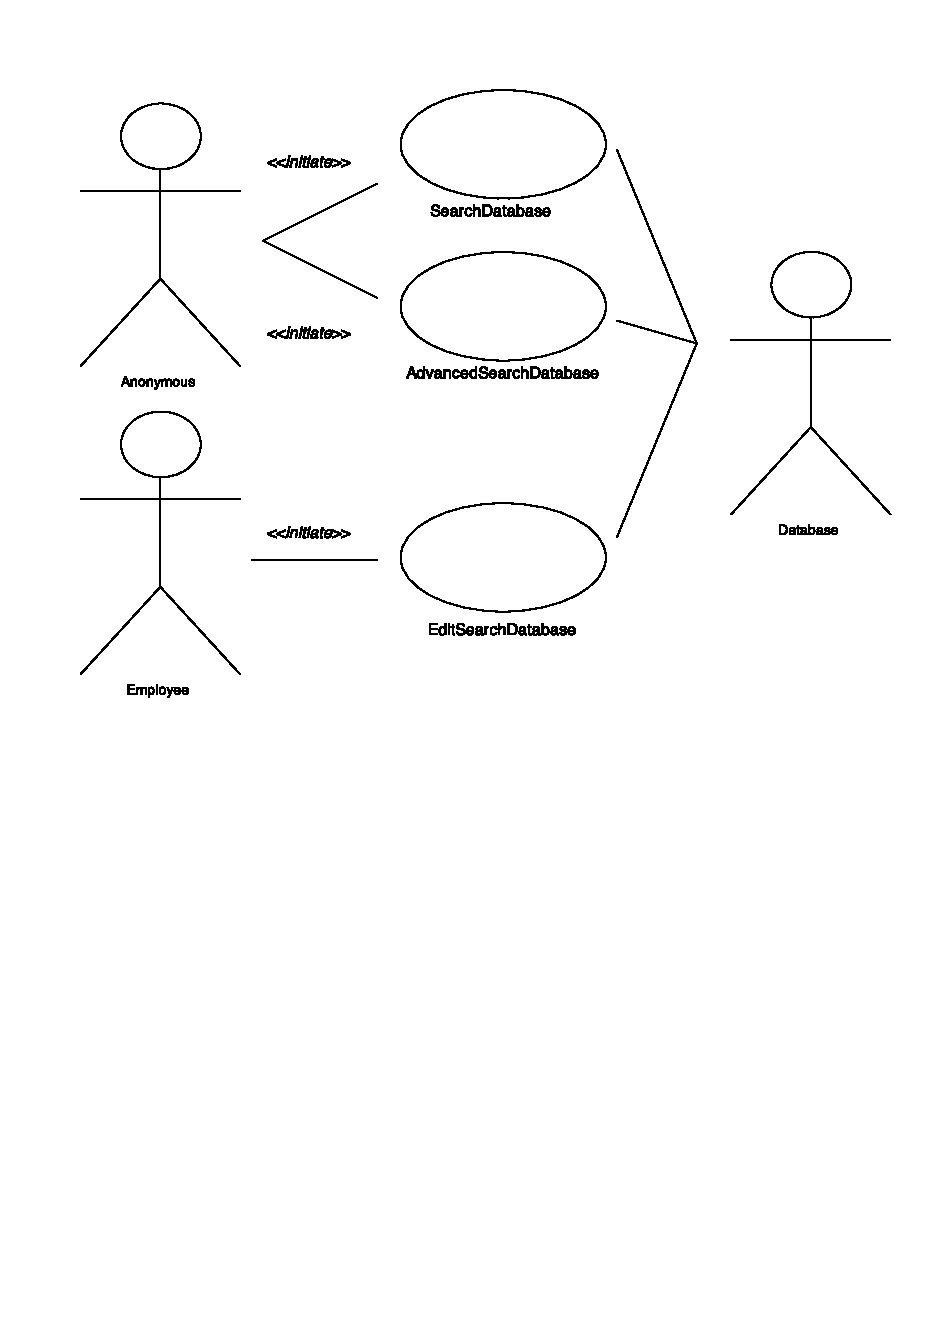
\includegraphics[height=120mm]{UseCase.pdf}

{\bf SearchDatabase}\\ 
Anonymous users use the search-engine and input a term in other to search the database and have the results they require displayed.
Searching the database does not require any special permissions.

{\bf AdvancedSearchDatabase}\\
Anonymous users use the advanced search-engine and input their search-terms into the fields representing the attributes they wish to match them against, in order to have the results they require displayed.
Searching the database does not require any special permissions.

{\bf EditDatabase}\\
An employee edits the database by accessing the edit-page through entering the necessary login credentials, modifies the database in which way desired and updates the database.
EditDatabase cannot be used without valid login credentials.\\
\vskip\medskipamount % or other desired dimension
\leaders\vrule width \textwidth\vskip0.4pt % or other desired thickness
\vskip\medskipamount % ditto
\nointerlineskip
The figure above is a use case model, which showcases the different possibilties of the product and to which kind of users they are available.

It is for instance evident through the model and the description of the functions, that any user will be able to search the database both in a basic and advanced way, where as only an employee with the necessary login credentials will be able to edit the entries in the database.
\newpage

\subsection{Specific Use Cases}

With the use case model created, we have an overview of the functional architecture of the website. With that in mind, we can explore some of the specific cases a bit further:\\

$\begin{array}{ll}
\hline
\text{Use Case Name}	& \text{SearchDatabase}\\
\hline
\text{Participating
	actors}	& \text{Initiated by Anonymous}\\
\hline
\text{Flow of events}	& \text{1. An anonymous user enters the website.}\\
& \text{2. The anonymous user enters the search-term into the search-field and presses send.} \\
& \text{3. The matching results are displayed.}\\
\hline
\text{Entry condition}	& \text{None}\\
\hline
\text{Exit conditions}	& \bullet \text{Anonymous exits the site.}\\
& \bullet \text{Anonymous submits a new search term.}\\
\hline
\end{array}$
\\

The above use case is the ordinary search of the database. It showcases in detail the specifics of the use case by displaying who initiates it, who, if any, it communicates with, the flow of the case itself as well as any conditions necessary.
We will now also inspect the remaining 2 use cases:\\

$\begin{array}{ll}
\hline
\text{Use Case Name}	& \text{AdvancedSearchDatabase}\\
\hline
\text{Participating
	actors}	& \text{Initiated by Anonymous}\\
\hline
\text{Flow of events}	& \text{1. An anonymous user enters the website.}\\
& \text{2. The anonymous user enters the search-terms into the fields of the matching attributes} \\
& \text{and presses send.}\\
& \text{3. The matching results are displayed.}\\
\hline
\text{Entry condition}	& \text{None}\\
\hline
\text{Exit conditions}	& \bullet \text{Anonymous exits the site.}\\
& \bullet \text{Anonymous submits a new search term.}\\
\hline
\end{array}$\\
\\
As we can see in the above case, no additional permissions/credentials are necessary to use the advanced search function.\\

$\begin{array}{ll}
\hline
\text{Use Case Name}	& \text{UpdateDatabase}\\
\hline
\text{Participating
	actors}	& \text{Initiated by Employee}\\
& \text{Communicates with Anonymous}\\
\hline
\text{Flow of events}	& \text{1. An employee user enters the website.}\\
& \text{2. The employee clicks on the edit hyperlink.} \\
& \text{3. The employee enters his/her login credentials.}\\
& \text{4. The employee enters required information and submits or deletes an entry}\\
\hline
\text{Entry condition}	& \bullet \text{Must have login credentials}\\
\hline
\text{Exit conditions}	& \bullet \text{Employee exits the site.}\\
& \bullet \text{Employee logs out.}\\
\hline
\end{array}$
\\

In this use case however, it's evident that in order to update the database, login credentials are needed. These are only to be provided to employees.
\newpage

\subsection{Class-diagram}

In order to grant an overview of the software-architecture, a class-diagram has been created:

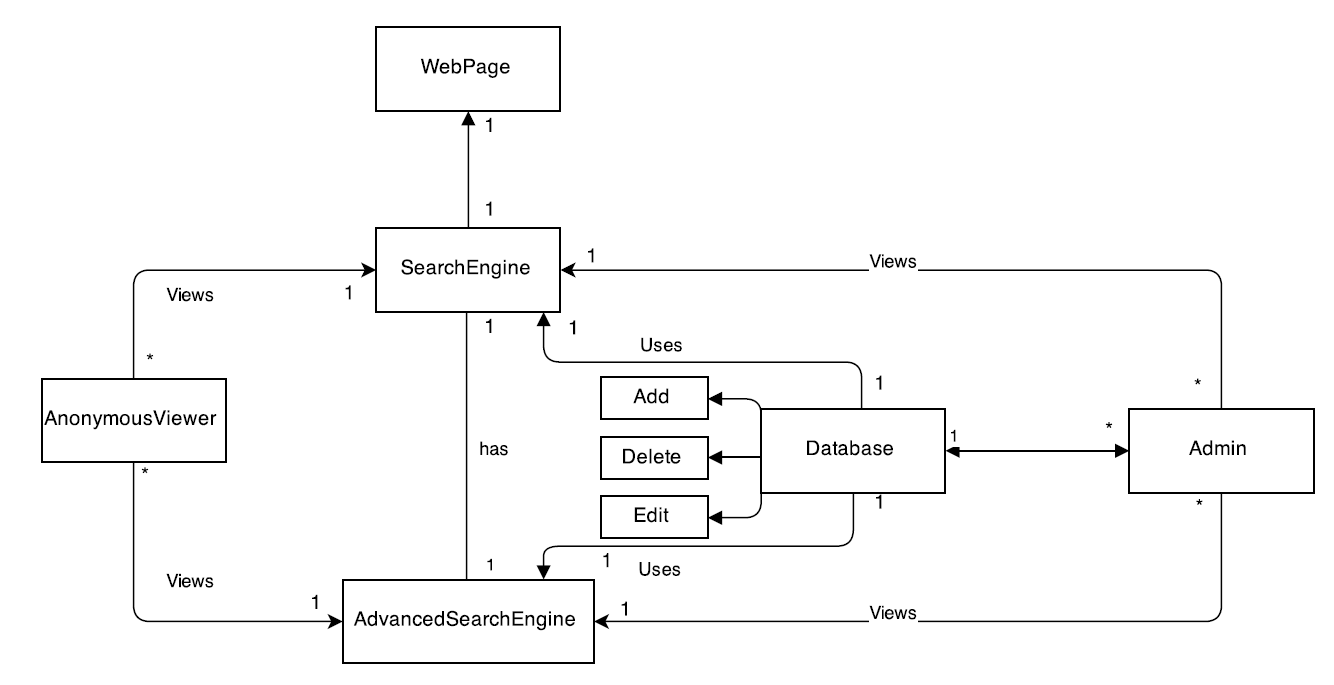
\includegraphics[height=90mm]{ClassDiagram.png}

The class-diagram shows the final product as a webpage offering 2 search-engines; one for basic and one for advanced searching.
Furthemore, the engines are linked to a database on the back-end, which is editable by administrators (employees), as they have the necessary login credentials. 
\newpage
\subsection{BCE-model}

To provide an easy reference-point for the different objects in our product and their respective responsibilities, a BCE-model has been created to effectively sort those objects into their representative categories.

\begin{gather*}
\begin{bmatrix}
\textbf{Boundary}&\textbf{Control}&\textbf{Entity}\\
Buttons&Search&Entries\\
Textfields&Advanced Search&Images\\
Headline&ImageClick\\
Background&Edit\\
\end{bmatrix}
\end{gather*}\\
\textbf{Boundary:}\\

Everything a user can see is a boundary object. In our case the buttons, search, advanced-search and edit, although also the text fields, the headline and the grey background.\\

\textbf{Entity:}\\

The entities here are all the information from the database, as well as the images that represent a specific set of information (an entry).\\

\textbf{Control:}\\

The search-button grabs the text input into the search-field and matches the term against the database.
The advanced search-button is similar except that it has 4 fields in which a user can match a term against specific attributes. 
Clicking on an image will take the user to a full-scale version of the image clicked.
Finally we have the edit button that allows an employee to change the entries in the database, or add/remove entries.
These are all control objects as they control one or more parts of the website's functionality.


\newpage
\subsection{Sequence-diagram}
We've already previously established different use cases relating to the project. Through these we can create sequence-diagrams illustrating them:

{\bf Use Case: SearchDatabase}\\

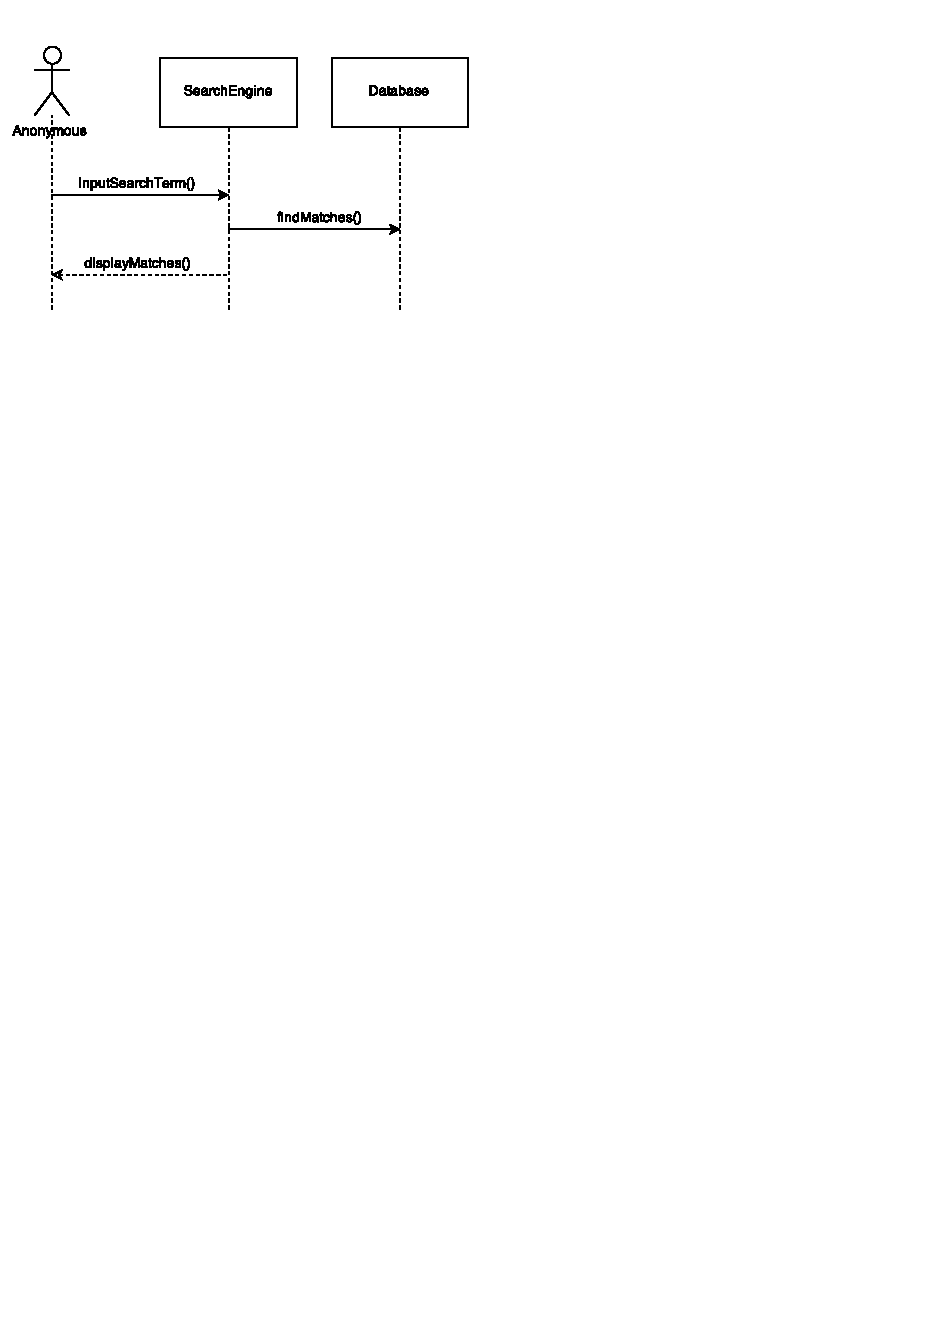
\includegraphics[height=92mm]{Sequence1.pdf}

{\bf Use Case: AdvancedSearchDatabase}\\

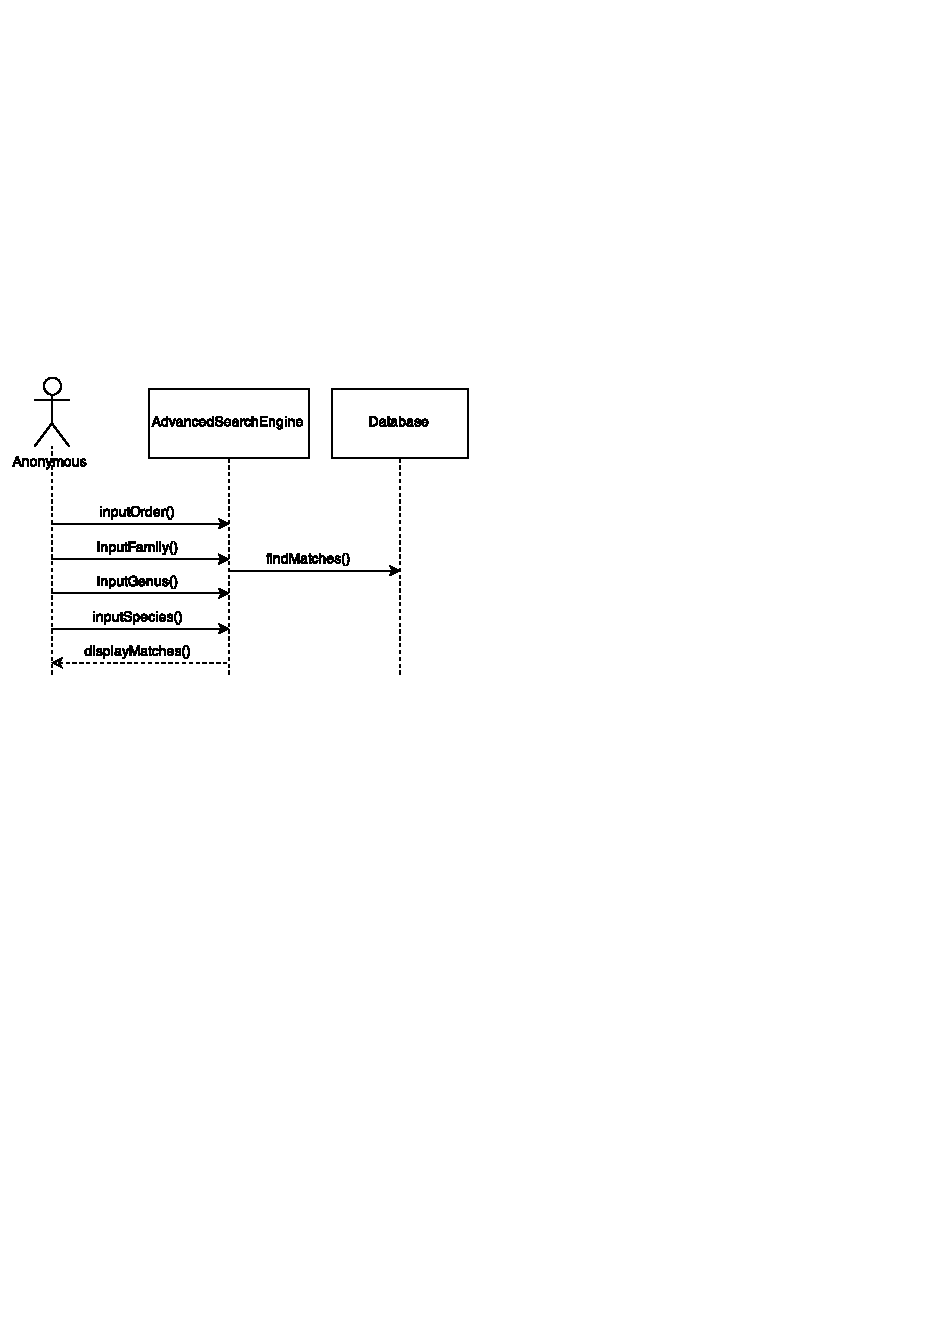
\includegraphics[height=92mm]{Sequence2.pdf}

{\bf Use Case: UpdateDatabase}\\

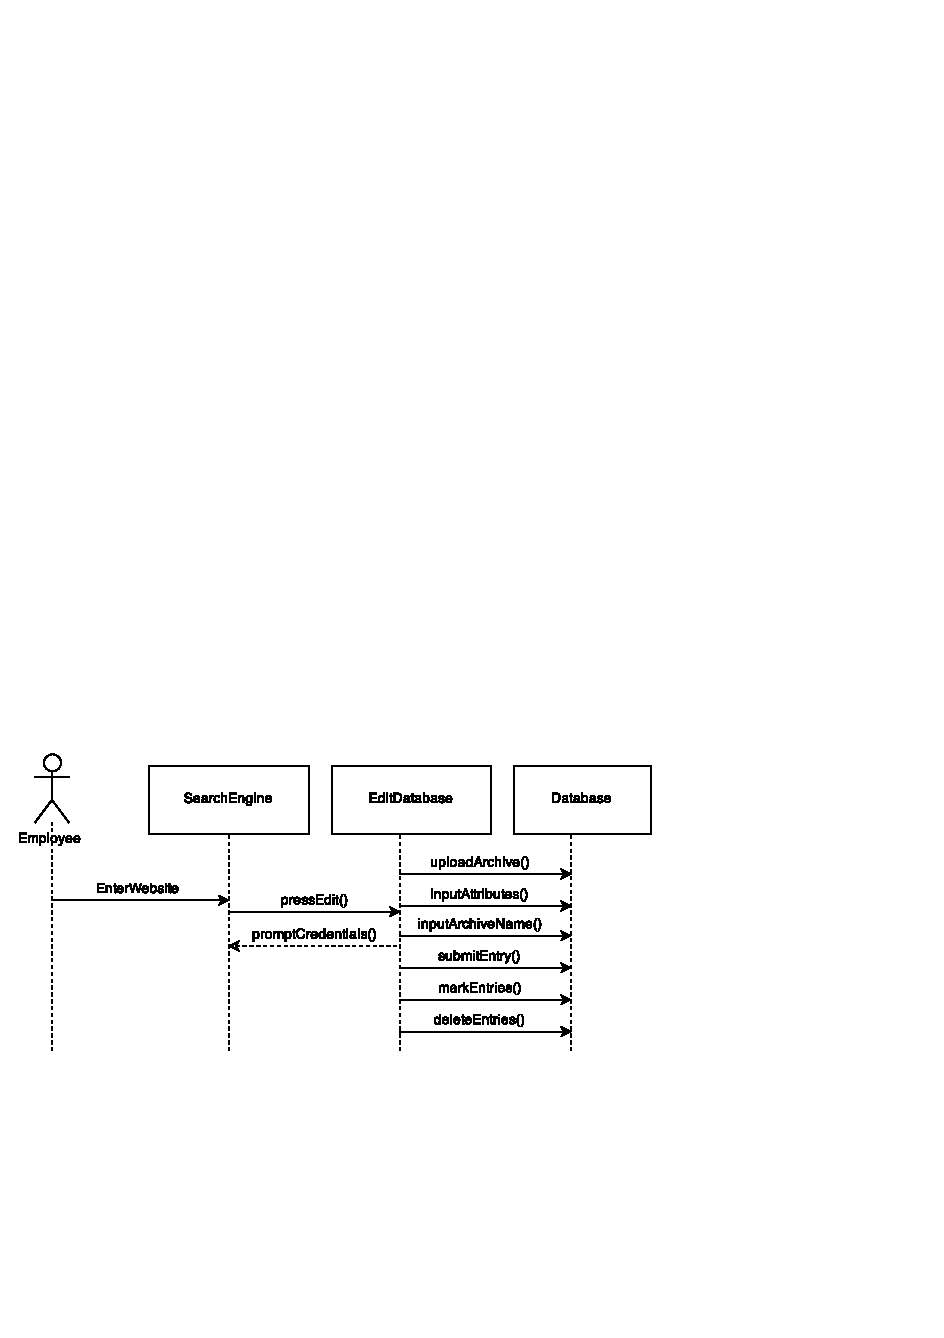
\includegraphics[height=92mm]{Sequence3.pdf}

\newpage

\section{System Design}
\subsection{Current Progress}

The Prototype of our product can be found and accessed at: \url{http://echiever.de/ProjectBeetle/Prototype3/prototype3.php}
\subsection{Summary}

At the current-stage of our product everything is fully functional.\\
The database consists of insect-entries, with order, family, genus, species, subspecies, description and the name of the .zip archive containing the high-resolution zoomify image of the insect as attributes.
Both the search-function and the advanced search-function are fully functional, and a method of displaying all existing entries in the database has been added (by simply searching for no term).
The database is now editable by either adding or deleting entries.\\
To add an entry you must now first upload an archive containing the zoomify image of an insect, and thereafter enter the appropriate information into its respective attributes, as well as enter the name of the archive which you uploaded.
Deleting an entry is done simply by marking a checkbox and clicking a delete-button.
At this point, all functional requirements have been fulfilled, and our work going forward is:
\begin{itemize}
\item Improve the design to better match that of the University of Hamburg's existing website
\item Implement any further wises the client may have
\end{itemize}
\newpage
\section{Testing}
\subsection{Search-engine test}

Testing the current edition of the product has gone to show that every of our newly implemented changes work as intended. We did however locate one problem, which is that logging out currently does appropriately delete the cookie responsible for checking whether you're logged in or not, and simply pressing 'return' after having logged out, will not re-prompt you for your credentials.

As for the current search, it now works with our updated database that includes the zoomify images.\\
The current search-able words in the normal search-engine are:

\begin{itemize}
	\item testFamily
	\item Sterrha
	\item Eilicrinia
\end{itemize}

As for testing the advanced search-engine, the following combination of terms and letters allow for full showing of its functionality.
\\\\
$
\begin{array}{c|c|c}
Order & Contains & stOr \\ 
Family & Starts with & test \\ 
Genus & Ends with & rha \\ 
Species & Contains & cord
\end{array}
$
\\

More in-depth descriptions of the various conducted tests are available as annexes at the end of the report.

\newpage
\section{Interaction and Design}
\subsection{Design}

In order to showcase the unit-interface of the product, a series of screenshots have been provided.

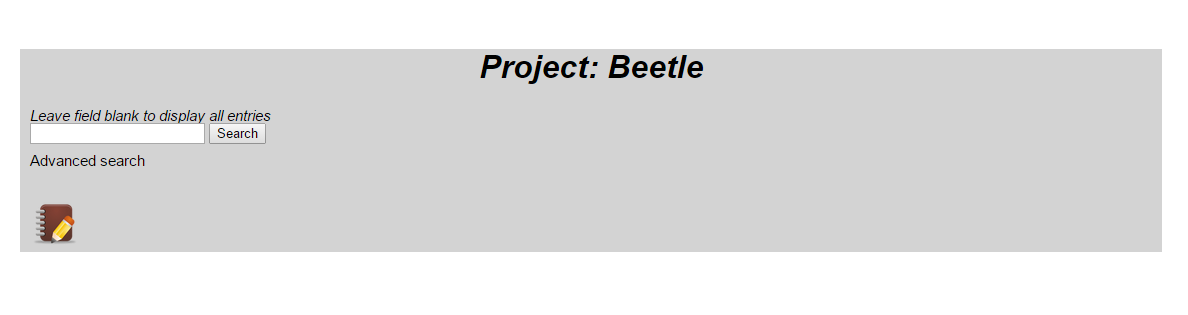
\includegraphics[height=45mm]{Beetle1.png}\\
Above is the frontpage of the website before any interaction has been done.\\
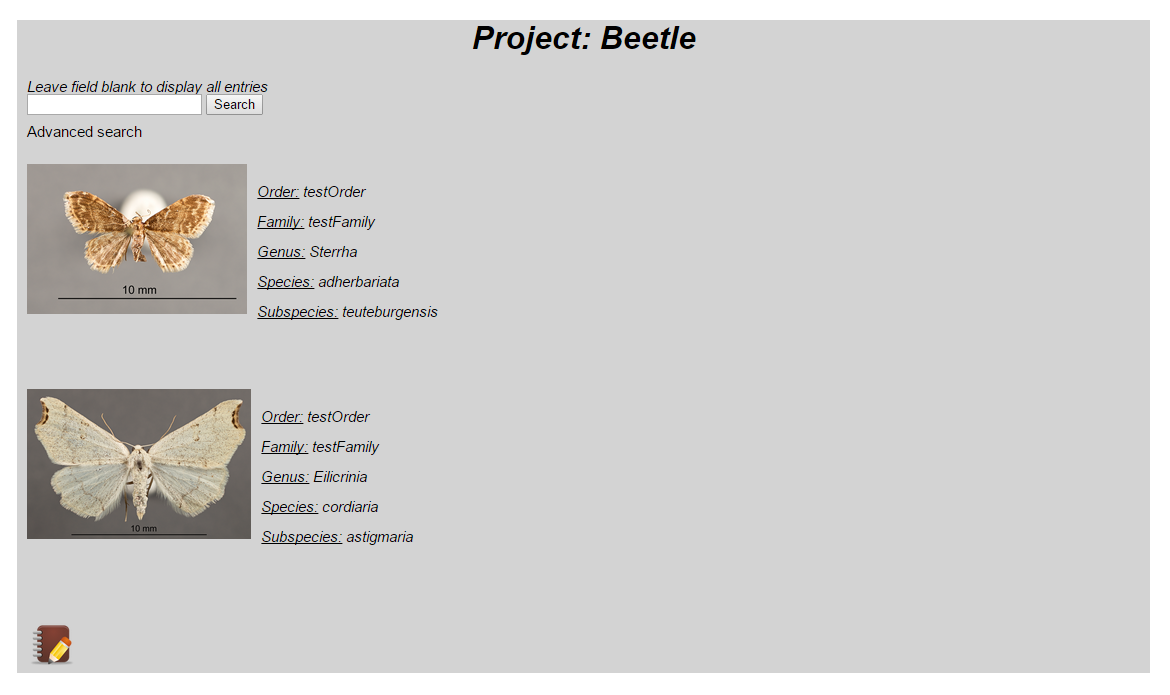
\includegraphics[height=100mm]{Beetle2.png}\\
Blank-search to display all entries.\\
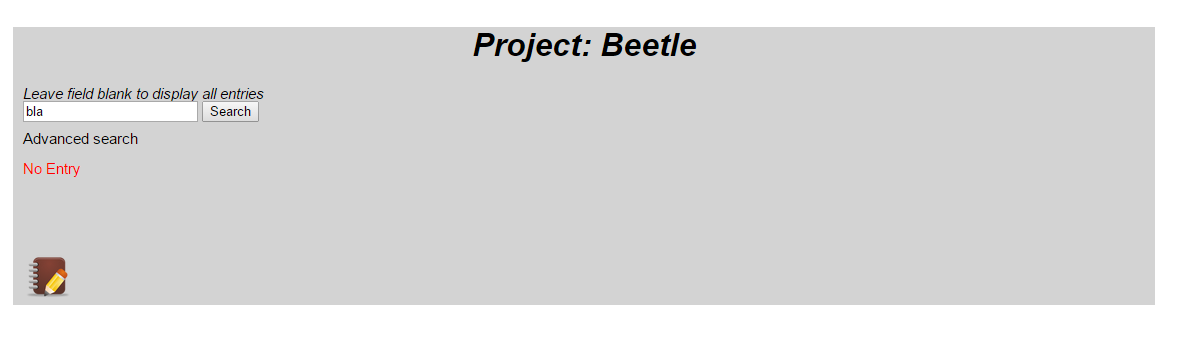
\includegraphics[height=45mm]{Beetle3.png}\\
No matching entries.\\
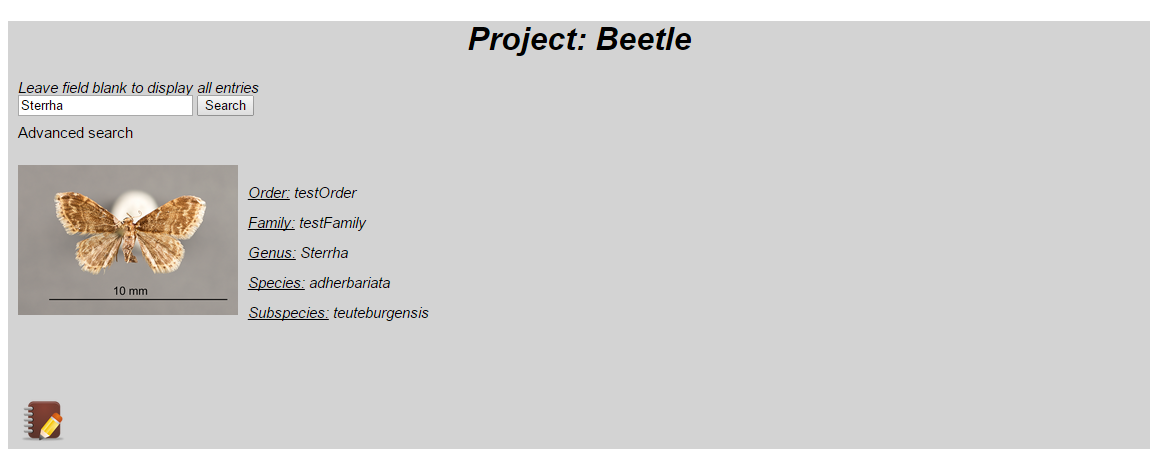
\includegraphics[height=70mm]{Beetle4.png}\\
Matching entry (entries).\\

\includegraphics[height=33mm]{Beetle5.png}\\
The advanced search-engine.\\

\includegraphics[height=45mm]{Beetle6.png}\\
No matching entries.\\
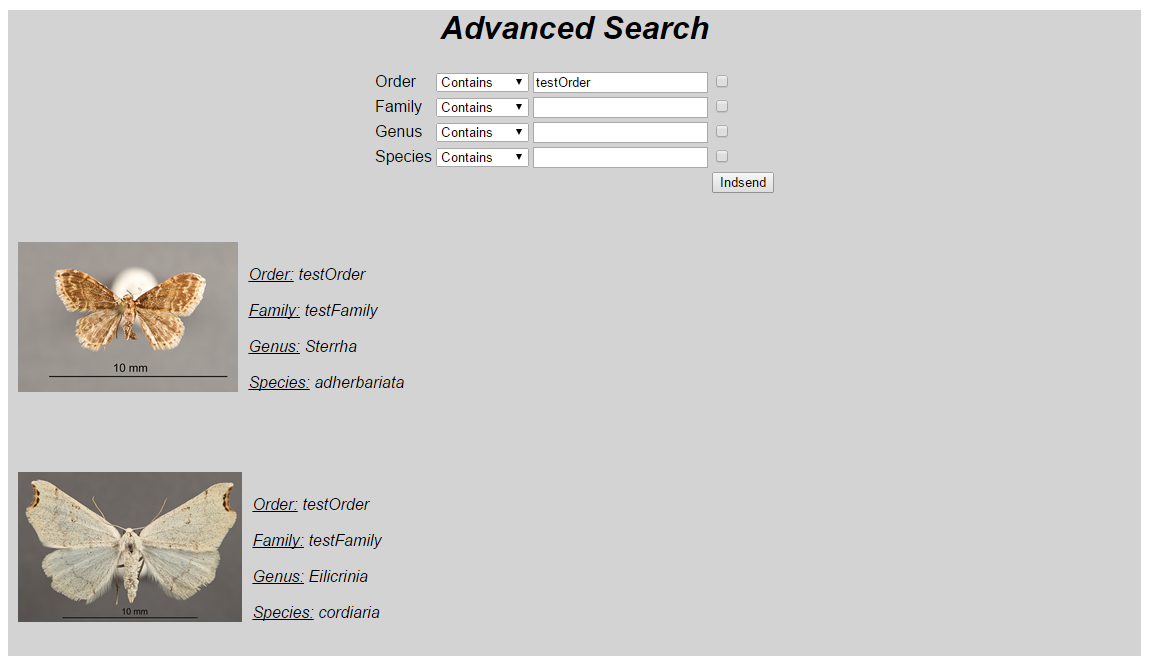
\includegraphics[height=90mm]{Beetle7.png}\\
Matching entry (entries).\\
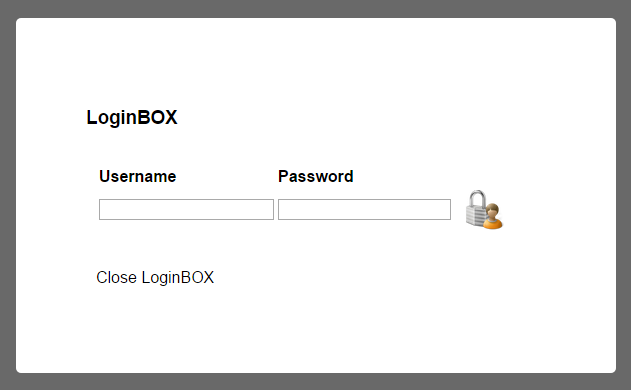
\includegraphics[height=60mm]{Beetle8.png}\\
Login function.\\
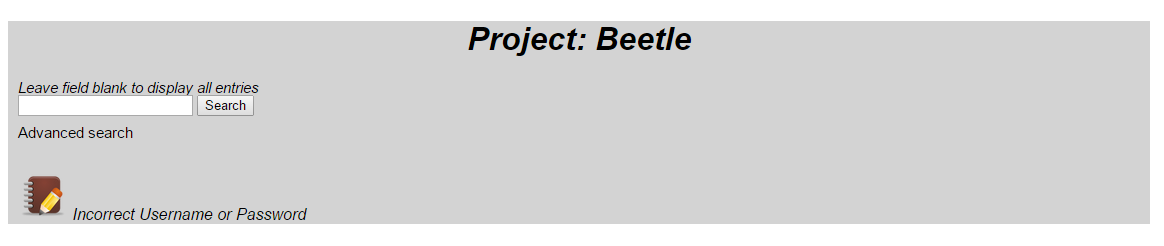
\includegraphics[height=60mm]{Beetle9.png}\\
Unsuccesful login.\\
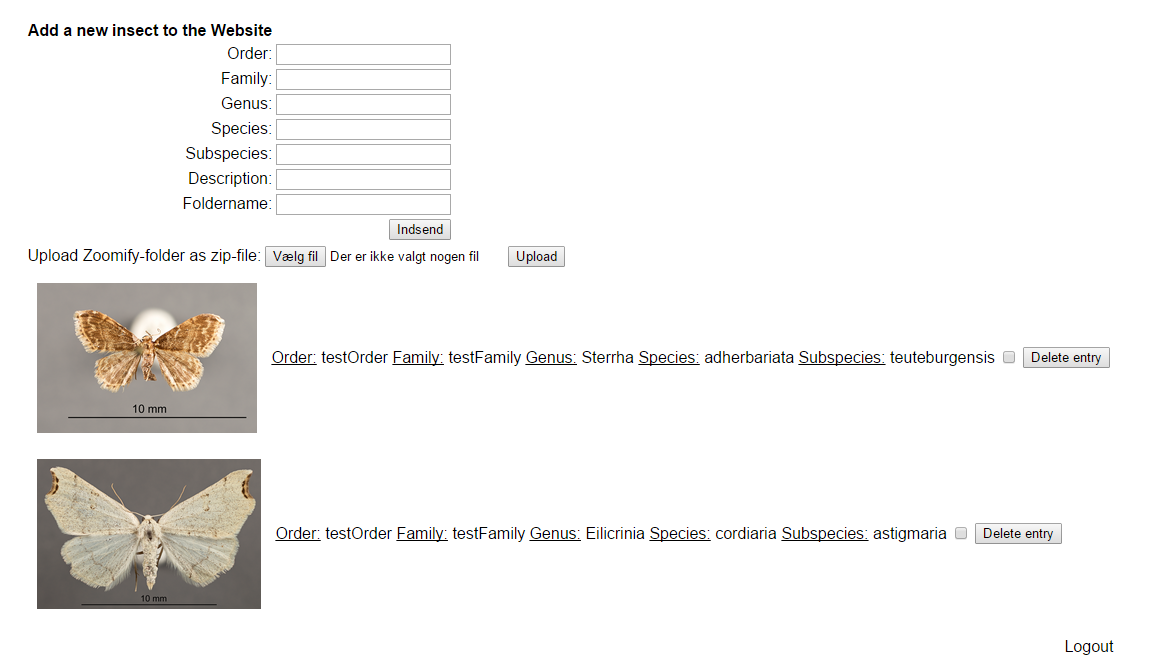
\includegraphics[height=100mm]{Beetle10.png}\\
Editing page displayed after succesful login.\\
\newpage

\section{Internal Cooperation}
\subsection{Summary}

{\bf 22nd of April:}

Come thus far, the cooperation of the University of Hamburg is satisfactory.\\
We have had a total of 2 "official" correspondences with our client in order to formally request server-access and the information we will be needing for the database. Furthermore we have been in contact with the University of Hamburg's Entomology department's representative after every work-session we have had, to present the current state of the product to him.
All the correspondonces have been fulfilling and we will be gaining access to the server as soon as their IT-department have created a user for us.\\ Furthermore, we will be receiving the necessary data for creating the proper database the 22th of April, after which we'll have everything we need. \\
The client also expressed satisfaction regarding the current state of our product, although a desire to have it looking more akin to the current layout of their website (which is only natural given that this is a prototype).\\
Our current way of work is based on us setting up workdays and meetings depending on necessity. This means that we, rather than using a gridlocked schedule, have been deciding on days to meet when the need was expressed.\\
For organisation we have been using a group created in Skype for communication as well as a repository in Github for file-access. \\
We have been internally communicating the progress of the product along the way and have also internally decided which partials have had the most importance at a given point in time, as to ensure we are all on the same page and that deadlines will be met.\\

So far we are making great progress in the development of the product itself, and we will soon have all the available means to ensure a succesful deliverance of a working product.\\
Our effort in organising meetings and working days has been less than ideal and together with our non-gridlock scheduling style have caused us to have many subsequent days of work, causing more of a burden than what is needed.\\
In order to make our developing from here on more efficient, more emphasis will be placed on proper scheduling, in order to spread out the workload and easen the burden on the entire group. This will also allow more time for quality control.\\
\newpage
{\bf 13th of May:}

At this stage the product is fully functional and everything that the University of Hamburg has desired, has been implemented.\\
In regards to our work we continued largely with the approach discussed in the summary from the 22nd of April, in the way that we have been setting up days on which we met and attempted to get as much work done as possible.\\
While we previously discussed the disadvantages to this approach, the progress we had made did not leave a lot of additional work to be completed, and therefore using a predetermined schedule was deemed unnecessary.\\
Our cooperation internally has been more than satisfactory, as each member of the group has been pulling their own assigned work-load, as well as having been constructive with input in regards to the whole project.\\
We have been working more closely with the University of Hamburg, showing them the development of the product underway, and have been continuously involving them in the whole process, so that they could provide their own input on the finished product.\\
The result is, that all their requests have been met satisfactorily, and that we are now almost ready to ship the finished product.

\newpage
\section{Litterature Reviews}
\subsection{Designing for usability - J.D. Gould and C. Lewis}
The text is based on the premise of three simple principles: Early focus on users, emphirical measurement and iterative design. The text is about system designs and how in the modern day everyone finds change very drastic. The designers and developers' jobs are to make everything easily accessible, and to create the system as something which can turn into a successor to old habits. \\
The fact that the article is from 1985 would in some people's minds be a signal of distress as the paper is 30 years old. What could designers 30 years ago possibly know about designing systems that we don't today? Especially considering the technology we work with? Well to our surprise the paper was very valid, even today. The principles which the paper state are things people may feel are intuitive and obvious. Even we thought so. But either way it is not to be forgotten that when you begin designing, you need to familiarise yourself with the potential users. The developer needs to think as a user and not as a developer. Creating something that seems easy for you might not seem as easy for others. The paper also emphasises the use of emphirical measurements. Developers tend to forget the purpose of testing publicly. Every type of person should be involved in the testing because of the fact that not all people may find using the given system easy. Presenting the system for new users/testers should also be done in such a manner that normal citizens can relate to why the system provides improvements. It is naive to only look at it in a rational matter, because doing so doesn't involve users at all. It is after all the users who are going to be using it. One cannot say that the users don't know what they want, they just need help understanding it. Why should the school system in Denmark start using programs like TI-Nspire and Maple, when a calculator and paper has worked for centuries? The argumentation and advantages need to be pointed out. Another good point the paper mentions is promises. Promising voice recognition and touch screen doesn't exactly mean that the device/system will be good quality. The design must be iterative, there is no advantage in locking the design at one state - it is only stubborn. Everything can be improved.
The paper, in short terms, focuses on the involvement of users and how the developers can involve more people. Changing habits is hard, but that doesn't mean it is impossible. 
\\
\\
This paper is relatable to our own project involving the University of Hamburg and their desire for a search-engine. Our approach so far hasn't really followed the principles to the fullest, but since we are so early in the developing process it doesn't matter that much as of yet. What we have done, is kept a constant contact with our client. After every session we ask the owner how he feels about our work. Our intended way of working is using the AGIL project management, where we make sure to be open to ideas, and try to implement the ideas the client asks for. What we maybe should consider is asking other users, since the owner might feel like it's a good idea, but his customers/users might not feel the same way. Even though we're only making a search-engine, which should be straight forward, we can't work with the premise that people can't have issues at this early stage. We certainly need to remember testing it with users of all sorts, going forward. User involvement is something we need to try and implement future work.
\newpage
\subsection{A Rational Design Process - David Lorge Parnas and Paul C. Clements}
This text is about a rational approach to designing a system. The idea is that you can't achieve one perfect result, but that you can fake it. Faking isn't seen as a bad thing in this situation. The idea is to do a lot of background work before the project coding commences. Today many coders usually utilise a "stream of consciousness" in which they realise an idea. The idea is then executed in a "stream of execution". In general this is a bad approach because the amount of time it would take to reach a result would be too long. That is why the paper recommends first making a requirements page in which you state what you, as a developer, can do and what the software has to include according to the customer. For instance which operating system the software has to work. Timing and accuracy constraints also help the developer set realistic goals and meet expectations. A probably worthwhile addition to a requirements document would also be changes likely to come up. This would not only make it easier for the developer long term, but also for newcomers who wish to improve the software. Another thing this paper urges new developers to do is to make sure documentation is proper and every step is documented. The paper urges developers to not have poor organisation, avoid "stream of consciousness” and not write excessive amounts of text when a shorter or more efficient paragraph could be used in place. Using confusing terminology should also be avoided - it is important to remember that even though you have lived inside this software for months, newcomers will be face-to-face with the software on a first time basis and not possess the knowledge you do. The small details are not as important as one would think - the bigger picture is considered more important.
The general idea is to use terms that are clear and easy to understand, using figures and expressions to make it all easier for newcomers to take in. The final document is not meant to be relaxing to read, but interesting. It should reward the reader with precise and detailed information.
\\
\\
The key element in our project is the documentation. There is a reason that we need to use more time on the document than on the code itself. The backbone to the whole project is the documentation. We try to implement as many figures as we possibly can. One thing we could work on is not using long phrases and sentences which seems to be a recurring element in our documents. Something we should consider implementing in our work in the future is requirements that are more precise. As of now, we usually decide where we are going whilst working. If we had something to work up to it would make the process much easier, and easier to see how much we actually are missing to reach the requirements. Besides, if the project is to be given to Hamburg, they would surely love to know the requirements for future developers to work and adjust to. We should try doing more rational design, as it would make our work easier in the future.
\newpage
\section{Annexes}

\subsection{Testing}
Test plan: \\
We want to test the general functionality of our product. The searchfunction is the most important part of the product, followed by the option to add an entry to the database. When those two functions work we can add more functions to the product, like the advanced search and the deletion of an entry in the database.\\\\
Test specification:\\
It should not be hard to test these functions, because we easily can test if the search gives the right output. The add and delete functionality should also be easy to test, because of its easy of use.\\
Testing the search could happen with the mentioned words and letters form section 5. Also we need to test the add entry and delete entry. Here we create a new entry, fitting to a Zoomify-image, and see if it works as intended. After that we could delete that entry again.\\\\
Test incident report:\\
Right now is there one bug in the code: If you login and logout, and go back in the browser you will go back to the edit page. Some could argue, that it is not that bad, because of the user has been logged in before already, but its still a bug that has to be fixed.\\\\
Test summary report:\\
We have tested our product a lot. But there is not much to test; a searchfield, an advanced-search, an add entry function and a delete entry function. Maybe you could count the add Zoomify-image in too, but we count it under the add function.\\
Until now did all tests work out fine. We could use the searches and get a working result. We could add and delete entries. And we could also add a new Zoomify-image-folder to the server.

\subsection{Github Log}
\noindent\makebox[\linewidth]{\rule{16.5cm}{0.4pt}}
a2f101f (HEAD, origin/master, origin/HEAD, master) Newest version of report 2.\\
0e78c2f timeline/new changelog\\
3628967 Reviews\\
af1ee59 okok\\
696e499 Added new changelog and code\\
7757964 Current state of the report.\\
f7b07df ChangeLog 20-21.04\\
298c0df cleanUP\\
5370d72 Mjallo virkelig ny\\
b0eee35 Mjallo ny\\
3045fee Mjallo\\
5726df9 Merge remote-tracking branch 'origin/master'\\
db797ee Fixed it!\\
8ee517f try tis\\
ebe615a Edited the report.\\
339fa41 Report + Pictures\\
0d21845 Delrapport 1- rettelse 1\\
c129a2c Killefilder\\
b0d9a30 Scheduleplan\\
c477a2f Skillmatrix\\
5751436 review of the review\\
6d0c506 Echo delrapport\\
0df006f Feedback til Project Echo\\
f2cdb65 .tex-filer 4 you\\
783af0a Redone the enviroment\\
16bfea5 English corrections/changes\\
5c8451d Changed the name\\
dd63eb0 Hermaen\\
6b0723b delrapport 1 assignments\\
be9faa6 1.6/1.8\\
0787272 Clean up!\\
00a6714 delete double\\
4f6a322 Projekt Etablering\\
d20a468 Rewrote the description\\
96050db Statements and Project Agreement Definition\\
da46259 Hello\\
4c5850d Initial Software Architecture (updated)\\
fa8824f Initial Software architecture\\
906e4ca Initial SPMP\\
0789c6f Introductory/Problem statement\\
acb4324 7.1 Deployment Diagram\\
bfcbd73 sup\\
9efec63 Revert "HEJ YUNUS"\\
13eef81 HEJ YUNUS\\
0851690 Hello Casper\\
\noindent\makebox[\linewidth]{\rule{16.5cm}{0.4pt}}

The code at this point in time have been developed in cooperation with the entire group through meetings at the school, where we worked on the code on only a single computer. As such, the Github log will not bear trace of editing of the code. The line 696e499 however shows the addition of the beta-version's code to the project's folder.

\subsection{Changelog}

	$$
	\begin{array}{lrl}
	\bf{Date} & \bf{Name} & \bf{Change} \\ 
	20-04-15 & YO/TD/EG/CL & Added~seachfield~and~\text{-}button \\
	20-04-15 & YO/TD/EG/CL & Added~database~and~entries \\
	20-04-15 & YO/TD/EG/CL & \vtop{\hbox{\strut \emph{Added~edit\-link}}} \\
	21-04-15 & YO/TD & \vtop{\hbox{\strut \emph{Added~Family\text{-},~Genus\text{-}~and~Species\text{-}names~form~the~database}}\hbox{\strut \emph{to~the~webpage}}} ~\\~
	21-04-15 & YO/TD & Added~picture~of~the~found~insect(s) \\
	21-04-15 & TD & Added~CSS\text{-}code~to~shine~the~webpage~a~bit~up \\
	21-04-15 & TD & Updated~the~database,~so~it~actually~shows~an~actual~insect\\
	21-04-15 & TD & Added~Order\text{-}name\\
	01-05-15 & TD & Added~Zoomify~pictures~and~the~description~of~the~insect\\
	01-05-15 & YO & Added~login\\
	11-05-15 & TD/CL & \vtop{\hbox{\strut \emph{	Added~option,~for~an~employee,~to~add~a~new~entry~into~}}\hbox{\strut \emph{the~database}}} \\
	11-05-15 & TD/CL & \vtop{\hbox{\strut \emph{	Added~option,~for~an~employee,~to~delete~an~old~entry~from}}\hbox{\strut \emph{the~database}}} \\
	11-05-15 & CL & \vtop{\hbox{\strut \emph{	Added~feature,~that~displays~all~entries,~when~the~search\text{-}}}\hbox{\strut \emph{~field~is~blank}}}\\
	11-05-15 & YO/EG & Added~functionality~for~the~advanced~search\\
	
	\end{array}
	$$
\subsection{Timeline}

	Initial custommer contact - {\bf 12th of March} - The custommer explained the desired functionality for the search-engine and their expectations of the outcome of the project. \\
	
	
	Report 1 - {\bf 21st of March} - The custommer received a copy of our first report, in order for them to view our progress and method of work.
	The custommer here expressed their desire for a more advanced option of using the search-engine. The exact specifics of what this should contain have not yet been stated, but they said they'd get back to us.
	They also expressed their desire for a dropdown menu showcasing all the entries in the database, in order to give the visitors a better overview.\\
	
	
	Prototype - {\bf 21st of April} - The custommer was officially shown the prototype of our search-engine, and they approved of its design. They pointed out some modifications that had to be made, most notably the correcting the attributes and wanting a new attribute, order, added. The correct order of attribute entries have now been specified as order, family, genus and species.\\
	
	Finished product - {\bf 11th of May} - On this date all functionality missing from the website was implemented and tested, so that we would end up with a product that (apart from a particular bug) is complete.\\
	It was also shown to the University of Hamburg, where they expressed great satisfaction with our product, and also the way we provided the option for displaying all entries, even prefering it to the one they had originally desired.\\



\end{document}
